\documentclass{beamer}
\usetheme{Singapore}
\usecolortheme{beaver}
\usepackage{subfig}
\usepackage{float}
\graphicspath{{./img/}}



\title{Hamiltonian Dynamics of Fluids}
\author{James Hawley}
\date{August 14, 2015}
\institute{University of Waterloo}


\begin{document}

	\begin{frame}
		\titlepage
	\end{frame}

	\section*{Contents}
		\begin{frame}{Contents}
			\tableofcontents
		\end{frame}

	\section{Background}
		\subsection{Hamiltonian Dynamics}
			\begin{frame}[t]{Classical Mechanics}
				\begin{columns}
					\begin{column}{0.5\textwidth}
						\begin{itemize}
							\item[]<2-> \textbf{Newtonian Dynamics}
							\item<3-> $\frac{d^2 \vec q}{dt} = -\nabla \Pi$
							\item<3-> Second order system
						\end{itemize}
					\end{column}
					\begin{column}{0.5\textwidth}
						\begin{itemize}
							\item[]<4-> \textbf{Hamiltonian Dynamics}
							\item<5-> $\frac{d \vec p}{dt} = -\frac{\partial H}{\partial \vec q}, \frac{d \vec q}{dt} = \frac{\partial \mathcal{H}}{\partial \vec p}$
							\item<5-> First order, coupled system
						\end{itemize}
					\end{column}
				\end{columns}
			\end{frame}
			\begin{frame}[t]{Fluids}
				\begin{columns}
					\begin{column}{0.5\textwidth}
						\begin{itemize}
							\item[]<2-> \textbf{Navier-Stokes Equations}
							\item<3-> $\rho\frac{d \vec u}{dt} = -\nabla p + \rho \nabla \Pi + F$
							\item<3-> Coupled, first order, nonlinear system
						\end{itemize}
					\end{column}
					\begin{column}{0.5\textwidth}
						\begin{itemize}
							\item[]<4-> \textbf{Hamiltonian}
							\item<5-> $\frac{d \vec p}{dt} = -\frac{\delta \mathcal{H}}{\delta \vec q}, \frac{d \vec q}{dt} = \frac{\delta \mathcal{H}}{\delta \vec p}$
							\item<5-> Coupled, first order, linear system
						\end{itemize}
					\end{column}
				\end{columns}
			\end{frame}
			\begin{frame}[t]{Hamiltonian Fluid Dynamics}
				\begin{itemize}
					\item[]<2-> System of PDEs $$\mathbf{0} = \textbf{F}\left(\mathbf{q}, \frac{\partial}{\partial x_i}, \frac{\partial}{\partial t} \right)$$
					\item[]<3-> is \emph{Hamiltonian} if $\exists \; \mathcal{H}, J$ such that
					\item[]<4->$$\mathcal{H} = \int_\Omega H(\mathbf{q}) d\mathbf{x}$$ is conserved, and solutions $\mathbf{q}(x_i, t)$ satisfy
					\item[]<5-> $$\mathbf{q}_t = \mathbf{J}\frac{\delta \mathcal{H}}{\delta \mathbf{q}}$$
				\end{itemize}
			\end{frame}
			\begin{frame}[t]{Derivatives}
				\begin{itemize}
					\item[]<2->$$ \mathcal{F}(\mathbf{q}) = \int_\Omega F(\mathbf{q}) \, d\mathbf{x} $$
					\item[]<3->$$ \lim_{\epsilon \rightarrow 0} \frac{\partial}{\partial \epsilon}\mathcal{F}(\mathbf{q} + \epsilon\delta\mathbf{q}) \equiv \left< \frac{\delta \mathcal{F}}{\delta \mathbf{q}}, \delta\mathbf{q} \right> \equiv \int_\Omega \frac{\delta \mathcal{F}}{\delta \mathbf{q}} \delta\mathbf{q} \, d\mathbf{x} $$
				\end{itemize}
			\end{frame}
			\begin{frame}[t]{Poisson Bracket}
				\begin{align*}
						\onslide<2->{\frac{\partial \mathcal{F}}{\partial t}}
						\onslide<3->{&= \int_\Omega \frac{\partial F}{\partial t} \, d\mathbf{x} \\}
						\onslide<4->{&= \int_\Omega \frac{\delta \mathcal{F}}{\delta \mathbf{q}}^\top \mathbf{q}_t\, d\mathbf{x} \\}
						\onslide<5->{&= \int_\Omega \frac{\delta \mathcal{F}}{\delta \mathbf{q}}^\top \mathbf{J}\frac{\delta \mathcal{H}}{\delta \mathbf{q}}\, d\mathbf{x} \\}
						\onslide<6->{&= \left< \frac{\delta \mathcal{F}}{\delta \mathbf{q}}, \mathbf{J}\frac{\delta \mathcal{H}}{\delta \mathbf{q}} \right> \\}
						\onslide<7->{&\equiv \{\mathcal{F}, \mathcal{H}\}}
					\end{align*}
			\end{frame}
			
		\subsection{Shallow Water Model}
			\begin{frame}[t]{Shallow Water Model}
				\begin{center}
					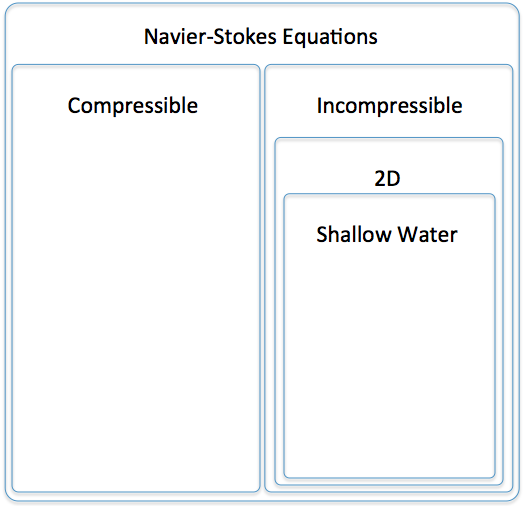
\includegraphics[width=0.4\textwidth]{nested_models_sw.png}
				\end{center}
			\end{frame}
			\begin{frame}[t]{Shallow Water Model}
				\begin{center}
					\begin{minipage}{0.45\textwidth}
						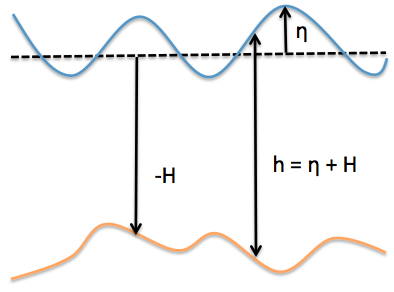
\includegraphics[width=\textwidth]{sw_diagram.png}
					\end{minipage}
					\begin{minipage}{0.45\textwidth}
						\begin{align*}
							0 &=\nabla \cdot \vec u\\
							0 &=\frac{\partial h}{\partial t} + \frac{\partial}{\partial x}(hu) + \frac{\partial}{\partial y}(hv)
						\end{align*}
					\end{minipage}
				\end{center}
			\end{frame}
		\subsection{Quasigeostrophic Model}
			\begin{frame}[t]{Geostrophic Model}
				\begin{center}
					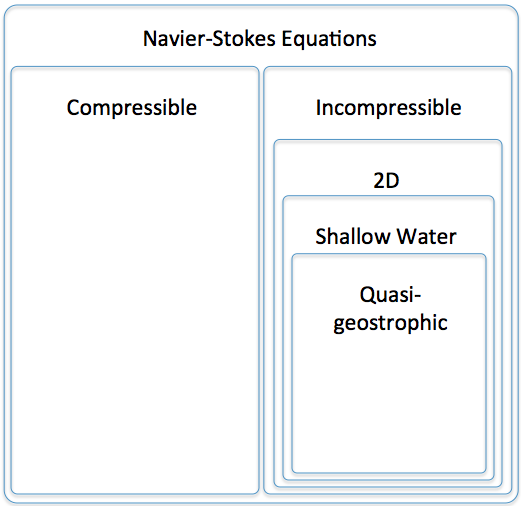
\includegraphics[width=0.4\textwidth]{nested_models_qg.png}
				\end{center}
			\end{frame}
			\begin{frame}[t]{Geostropic Model}
				\begin{align*}
					\frac{d \vec u}{dt} + 2 \vec \Omega \times \vec u &= -\frac{\nabla p}{\rho} + \nabla \Pi + \frac{F}{\rho}\\
					\vec u &= \text{velocity field}\\
					\vec \Omega &= \text{rotation vector}\\
					p &= \text{pressure}\\
					\Pi &= \text{scalar potential field}\\
					F &= \text{viscous forces}\\
				\end{align*}
			\end{frame}
			%--- Next Frame ---%
			\begin{frame}[t]{Quasigeostrophic Model}
				\begin{center}
					\begin{align*}
						0 &=\frac{\partial q}{\partial t} + J(\psi, q) \\
						J(a, b) &=\frac{\partial a}{\partial x}\frac{\partial b}{\partial y} - \frac{\partial a}{\partial y}\frac{\partial b}{\partial x} \\
					\end{align*}
				\end{center}
			\end{frame}

	\section{Main Work}

	\section{References}
		\begin{frame}{References}
			\begin{enumerate}
				\item Reference
			\end{enumerate}
		\end{frame}

\end{document}
